\section{Establishing Connectivity}
\begin{mytitle}[How to connect UbiComp functionality?] We can connect on three levels: on the physical and medium access layer via low-power wireless, on the network level via internet of things (IoT) and on the application layer via web of things (WoT).
\end{mytitle}

\subsection{Low-Power Wireless}
\begin{mytitle}[Wireless communication]
    \begin{mysubtitle}[Wireless communication benefits]\hfill
    \begin{itemize}
        \item Supports mobility
        \item Less infrastructure
    \end{itemize}
    \end{mysubtitle}
    \begin{mysubtitle}[Wireless communication drawbacks]\hfill
    \begin{itemize}
        \item Typically lower transmission rates
        \item Restrictive regulation of resources
        \item Lower security
        \item Higher loss rates
        \item Higher power consumption
    \end{itemize}
    \end{mysubtitle}
\end{mytitle}
\begin{mytitle}[Energy harvesting] We can harvest power directly from switching events. A spring in a switch outputs enough energy to transmit three identification messages. Other sources of energy include wrist-watches, photovoltaic, piezoelectricity, pyroelectricity, atmospheric pressure changes and other ambient radiation.
\end{mytitle}
\begin{mytitle}[Wi-Fi (802.11)] Wi-Fi is a power-consuming communication system, therefore there is no wide adaptation in the sensor network and IoT space. Instead they rely on 802.15.4 (a standard for low-rate WPANs) and bluetooth low energy (BLE).
\end{mytitle}
\begin{mytitle}[Passive Wi-Fi] Passive Wi-Fi uses backscatter communication to generate up to 11 Mbit/s transmissions and has 3-4 orders of magnitude lower energy consumption. It works by offloading RF componenets to a single plugged-in device in the network, creating a single-frequency tone. Passive Wi-Fi devices communicate by reflecting this tone via a digital switch. Those transmissions can be decoded by all devices within a Wi-Fi chipset. The range is typically 10-100 m.
\end{mytitle}
\begin{mytitle}[Interscatter] Interscatter describes the modulation of the reflection of a BLE packet to generate a Wi-Fi packet.
\end{mytitle}
\begin{mytitle}[Ultra-low-power communication] The core idea is to exploit energy asymmetries. Every sensor node has very little power but there is a sink node with lots of power.
    \begin{mysubtitle}[Low-power listening (LPL)] The receivers periodically turns on the radio and polls the medium.
    \end{mysubtitle}
    \begin{mysubtitle}[Low-power probing (LPP)] The receivers periodically send probes, the sender listens for them and sends payload immediately after receiving one.
    \end{mysubtitle}
\end{mytitle}
\begin{mytitle}[Multiplexing] The goal here is to make best use of the precious shared wireless medium.
    \begin{mysubtitle}[Space division mutltiple access (SDMA)] Here we segment space into cells/sectors. We use the same frequencies in different cells. The advantage is its simplicity. The disadvantages are the needed infrastructure investment and handover management.
    \end{mysubtitle}
    \begin{mysubtitle}[Frequency division multiple access (FDMA)] Here we separate the spectrum into smaller frequency bands and allocate one band per channel. The advantage is that there is no need for co-ordination. The disadvantages are the possible waste of bandwidth and its inflexibility.
    \end{mysubtitle}
    \begin{mysubtitle}[Time division multiple access (TDMA)] Here one channel gets the entire spectrum but only for a short period of time. The advantages are that we use only one carrier at at time and that there is higher throughput possible. The disadvantage is the precise synchronization that is needed.
    \end{mysubtitle}
    \begin{mysubtitle}[Combination of FDMA + TDMA (+ SDMA)] A combination has the advantages that it is more robust against selective interference and has better eavesdrop resistance. The disadvantage is the precise synchronization that is needed.
    \end{mysubtitle}
    \begin{mysubtitle}[Code division multiple access (CDMA)] Here we take a narrowband signal and spread it over the available spectrum. All channels then use the same spectrum simultaneously and statistical methods are used to disentangle the signals. Each channel has a unique code. In DS-CDMA the code is used to chip the signal into smaller pieces, while in FH-CDMA the code is used as a hopping pattern between frequencies. The advantages here are its bandwidth efficiency, that no synchronization is needed and its robustness against interference and eavesdropping. The disadvantage is that more complex signal filtering is needed for decoding the signals.
    \end{mysubtitle}
\end{mytitle}
\begin{mytitle}[Low-power wide area network (LPWAN)] We want long range, a low number of base stations, a low data rate, low battery and low subscription costs. Examples of LPWAN providers are SigFox and LoRa.
\end{mytitle}

\subsection{Bluetooth}
\begin{mytitle}[Bluetooth] Bluetooth is intended as a WLAN replacement in personal area networks. It is much smaller, cheaper and needs less power, but only has a short range ($\sim$10 m) and up to 720 kb/s. It also needs a complex communication stack to support voice and data as well as bluetooth profiles for different device functions. 
\end{mytitle}
\begin{center}
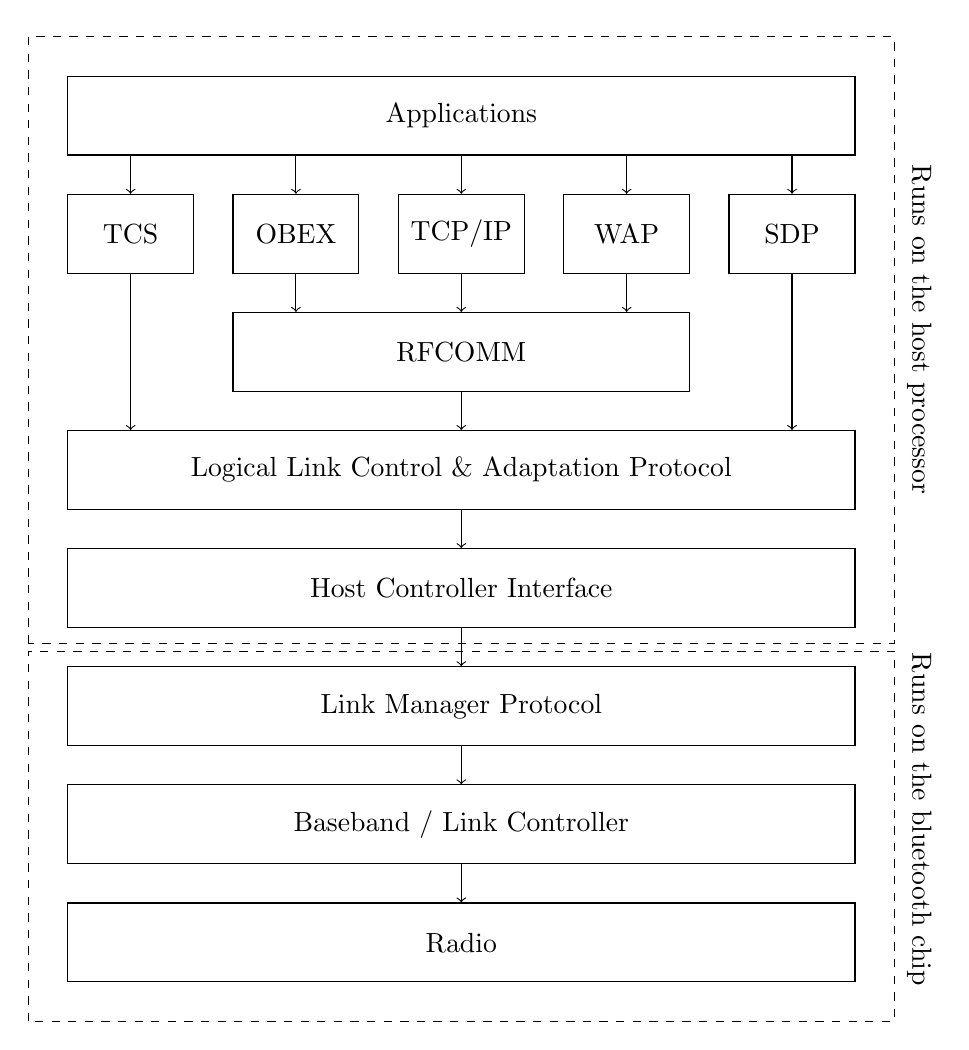
\begin{tikzpicture}

\node (A) at (5,-1) [draw,minimum width=10cm,minimum height=1cm] {Radio};
\node (B) at (5,0.5) [draw,minimum width=10cm,minimum height=1cm] {Baseband / Link Controller};
\node (C) at (5,2) [draw,minimum width=10cm,minimum height=1cm] {Link Manager Protocol};
\node (D) at (5,3.5) [draw,minimum width=10cm,minimum height=1cm] {Host Controller Interface};
\node (E) at (5,5) [draw,minimum width=10cm,minimum height=1cm] {Logical Link Control \& Adaptation Protocol};
\node (F) at (5,6.5) [draw,minimum width=5.8cm,minimum height=1cm] {RFCOMM};
\node (G1) at (0.8,8) [draw,minimum width=1.6cm,minimum height=1cm] {TCS};
\node (G2) at (2.9,8) [draw,minimum width=1.6cm,minimum height=1cm] {OBEX};
\node (G3) at (5,8) [draw,minimum width=1.6cm,minimum height=1cm] {TCP/IP};
\node (G4) at (7.1,8) [draw,minimum width=1.6cm,minimum height=1cm] {WAP};
\node (G5) at (9.2,8) [draw,minimum width=1.6cm,minimum height=1cm] {SDP};
\node (H) at (5, 9.5) [draw,minimum width=10cm,minimum height=1cm] {Applications};

\draw [->] (G1 |- H.south) -- (G1);
\draw [->] (G2 |- H.south) -- (G2);
\draw [->] (G3 |- H.south) -- (G3);
\draw [->] (G4 |- H.south) -- (G4);
\draw [->] (G5 |- H.south) -- (G5);
\draw [->] (G1.south) -- (G1 |- E.north);
\draw [->] (G2.south) -- (G2 |- F.north);
\draw [->] (G3.south) -- (G3 |- F.north);
\draw [->] (G4.south) -- (G4 |- F.north);
\draw [->] (G5.south) -- (G5 |- E.north);
\draw [->] (F) -- (E);
\draw [->] (E) -- (D);
\draw [->] (D) -- (C);
\draw [->] (C) -- (B);
\draw [->] (B) -- (A);

\draw [dashed] (-0.5, 2.8) rectangle (10.5, 10.5) node [label={[label distance=1.5cm,text depth=3ex,rotate=-90]right:Runs on the host processor}] {};
\draw [dashed] (-0.5, -2) rectangle (10.5, 2.7) node [label={[label distance=-0.1cm,text depth=3ex,rotate=-90]right:Runs on the bluetooth chip}] {};

\end{tikzpicture}
\captionof{figure}{Classic Bluetooth protocol stack}
\end{center}
\begin{mytitle}[Frequency hopping on the radio layer] If a collision occurs, a packet is retransmitted on a different channel. The specific hopping pattern is not known to outsiders. A common hopping sequence for all cooperating devices is determined by the baseband layer. There are about 1600 hops/s.
\end{mytitle}
\begin{mytitle}[Baseband]
    \begin{mysubtitle}[Addressing] Each bluetooth device has a 48 bit device ID. There is a 3 bit active member address (AMA) when it is active in a piconet and an 8 bit parked member address (PMA) when it is not active. A piconet consists of bluetooth units sharing a single frequency-hopping channel. A single master connects to a maximum of 7 slaves due to the 3 bit address. Communication is point-to-point master-slave or multicast from the master to all of its slaves.
    \end{mysubtitle}
    \begin{mysubtitle}[Connection states] There are 7 different states:
    \begin{itemize}
        \item Standby: not participating in a piconet
        \item Inquiry: learn about identity of other devices around
        \item Page: invitation to a known device to join
        \item Active: full power mode, listening to all packets
        \item Sniff: low power mode, wakes up every x ms to check
        \item Park: low power mode, only listens to sync beacons, not used anymore
        \item Hold: low power mode, master puts device on hold, slave returns automatically
    \end{itemize}
    \end{mysubtitle}
    \begin{mysubtitle}[Packet Format] 72 bits access code, 54 bits header, 0-2745 bits payload
    \end{mysubtitle}
    \begin{mysubtitle}[Error Handling]\hfill
    \begin{itemize}
        \item Automatic repeat request (ARQ): determined from 1-bit ACK/NAK and 1-bit seq. number
        \item Forward error correction (FEC): reduces number of repeat requests but adds overhead
    \end{itemize}
    \end{mysubtitle}
\end{mytitle}
\begin{center}
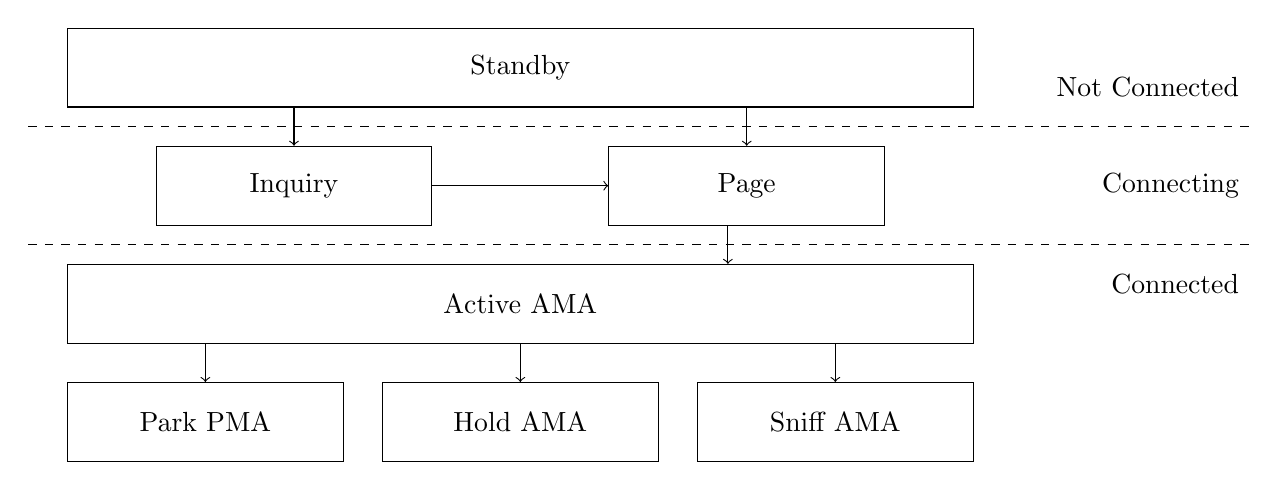
\begin{tikzpicture}

\node (A) at (5.75,4.5) [draw,minimum width=11.5cm,minimum height=1cm] {Standby};
\node (B1) at (2.875,3) [draw,minimum width=3.5cm,minimum height=1cm] {Inquiry};
\node (B2) at (8.625,3) [draw,minimum width=3.5cm,minimum height=1cm] {Page};
\node (C) at (5.75,1.5) [draw,minimum width=11.5cm,minimum height=1cm] {Active AMA};
\node (D1) at (1.75,0) [draw,minimum width=3.5cm,minimum height=1cm] {Park PMA};
\node (D2) at (5.75,0) [draw,minimum width=3.5cm,minimum height=1cm] {Hold AMA};
\node (D3) at (9.75,0) [draw,minimum width=3.5cm,minimum height=1cm] {Sniff AMA};

\draw [->] (B1 |- A.south) -- (B1);
\draw [->] (B2 |- A.south) -- (B2);
\draw [->] (B1) -- (B2);
\draw [->] ([xshift=7.5em]C |- B2.south) -- ([xshift=7.5em]C.north);
\draw [->] (D1 |- C.south) -- (D1);
\draw [->] (D2 |- C.south) -- (D2);
\draw [->] (D3 |- C.south) -- (D3);

\draw [dashed] (-0.5,2.25) -- (15,2.25);
\draw [dashed] (-0.5, 3.75) -- (15,3.75);

\node at (15, 4.25) [anchor=east] {Not Connected};
\node at (15, 3) [anchor=east] {Connecting};
\node at (15, 1.75) [anchor=east] {Connected};

\end{tikzpicture}
\captionof{figure}{Baseband Connection States}
\end{center}

\begin{mytitle}[Link manager] The link manager manages the piconet, authentication (only accept connections from trusted devices), switching of master/slave roles and the tearing down of connections when slaves leave. It also handles the low power modes. Active voice mode uses around 10 mA, active data mode uses around 6 mA and hold/park mode only 60 $\mu$A. For comparison bluetooth low energy has a 1 $\mu$A average.
\end{mytitle}
\begin{mytitle}[Logical link control \& adaptation protocol (L2CAP)] L2CAP adapts the upper layer protocols to the baseband. It handles the segmentation and reassembly of the upper layer protocol packets and the protocol multiplexing over a single air interface.
\end{mytitle}
\begin{mytitle}[Radio frequency communication (RFCOMM)] RFCOMM emulates a serial port and thus allows multiple "ports" over a single bluetooth channel. This enables TCP/IP and roughly the same service and reliability guarantees as TCP.
\end{mytitle}
\begin{mytitle}[Bluetooth low energy (BLE)] BLE has up to 260 Kbps data rate and only sends occasional updates of sensor values. It does not have voice support, has fewer but broader channels, has a faster connection setup and the modulation scheme is optimized for low power usage.
\end{mytitle}
\begin{mytitle}[Generic attribute profile (GATT)] GATT is the BLE application-layer protocol that reads and writes remote variables, the length of which typically ranges between 20 and 40 bytes. Related characteristics are grouped into services (based on GATT) like "Device information service", "Heart rate profile", etc. The central device is the GATT client while the peripheral devices are GATT servers. Peripheral-peripheral communication is possible through abstractions managed by the central device.
\end{mytitle}
\begin{mytitle}[IPv6-based LPWANs] These want direct end-to-end internet integration of resource-constrained embedded devices. Edge routers are used to connect the LoWPAN to the IP infrastructure. An example provider is 6LoWPAN, which transports IPv6 packets over BLE while recognizing and implementing BLE's limits on protocol overhead. A border router connects LWPANs to IP infrastructure, performs (de-)compression and disseminates routing information.
\end{mytitle}

\subsection{Internet of Things}
\begin{mytitle}[Transmission control protocol (TCP)] TCP establishes connectivity between processes. 
    \begin{mysubtitle}[Three-way handshake] SYN, SYN-ACK, ACK
    \end{mysubtitle}
    \begin{mysubtitle}[Sequence number and ack number] These numbers enable the in-order delivery of packets
    \end{mysubtitle}
    \begin{mysubtitle}[Window] Windows are the limit on packets that can be "in flight" simultaneously
    \end{mysubtitle}
    \begin{mysubtitle}[Flow control] Flow control makes sure that networks are not overloaded. AIMD is the classic flow control implementation.
    \end{mysubtitle}
\end{mytitle}
\begin{mytitle}[User datagram protocol (UDP)] UDP is used by applications that do not require the reliability of TCP. It is much more leightweight as there is no connection setup and little overhead.
\end{mytitle}
\begin{mytitle}[Representational state transfer (REST)] REST provides architectural guidelines for computing infrastructure, including the web. It is a resource-oriented architecture (ROA), meaning that the functionality is integrated into resources, not offered by services. 
    \begin{mysubtitle}[Constraints] REST contstraints include the separation of concerns through a client-server model (decoupling and evolvability), stateless interactions (decoupling and scalability), cacheability (scalability and performance), layered systems (scalability) and uniform interfaces (decoupling and evolvability).
    \end{mysubtitle}
\end{mytitle}
\begin{myremark} In REST, there is state in resources and in the client, but not in the transaction. This enables that a series of interactions by a client can be handled by different servers.
\end{myremark}
\begin{mytitle}[Web resources] A web resource is "anything that you want to talk about", like products, categories, customers, shopping carts, etc. but also client state transitions like next links and paged results.
\end{mytitle}
\begin{myremark} In HTTP, verbs stay polymorphic, i.e. we use GET for all types of resources. In contrast RPC-style WS$^*$-web services define operations specific for object types.
\end{myremark}
\begin{mytitle}[Shared representation model]Every web browser can access every web resource because HTTP works the same for every resource. Interacting with the resource is possible without knowing it beforehand. The representations that are exchanged depend on a shared representation model.
\end{mytitle} 
\begin{mytitle}[Resource representations] Resources are abstract entities, interaction with resources happens via resource representations. Representation formats can be negotiated between peers and it is communicated which kind of representation is used. When you access a web resource, you see one of its representations your browser negotiates for you. Resource representations contain links to identified resources. Servers guide interactions by providing links. Links are possible state transitions of the client/server application.
\end{mytitle}

\subsection{Web of Things}
\begin{mytitle}[IoT vs WoT] IoT describes the global network of physical objects that communicate using the internet protocol. WoT refers to a specific part of the WWW where physical entities are identified by URLs and interlinked by hyperlinks.
\end{mytitle}
\begin{mytitle}[Hypermedia as the engine of application state (HATEOAS)] With HATEOAS, a machine API needs no syntactic documentation. Making full use of the WoT (including HATEOAS) for devices and services facilitates the autonomous usage of their interface by machine clients and the creation of flexible mashups across services by different providers. HATEOAS makes systems flexible and robust by decoupling clients and servers as clients discover state transitions at runtime.
\end{mytitle}
\begin{mytitle}[HTTP] HTTP is a text-based protocol. HTTP requests indicate the action to be performed and what type of response the client will accept. The advantages are that it is understandable and debuggable. The disadvantage is that it is not very efficient. 
\end{mytitle}
\begin{mytitle}[The constrained application protocol (CoAP)] CoAP is an alternative to HTTP, targeted to constrained nodes and networks. Constrained nodes can be sensors with limited memory and processing power and constrained networks can be slow, unreliable and intermittent. CoAP is optimized for bandwidth and processing efficiency. It is based on UDP and has lightweight security. In CoAP, the client can send an observe to the server, then it will get notifications about resource state changes. There also exists support for multicast. Security in CoAP emulates a 3-way handshake. For low-power devices there is still ongoing work.
    \begin{mysubtitle}[Message types] There are four message types in CoAP:
    \begin{itemize}
        \item Confirmable (CON): reliable message with retransmission
        \item Non-Confirmable (NON): best effort transmission
        \item Acknowledgement (ACK): confirms a CON message
        \item Reset (RST): used when CON or NON cannot be processed
    \end{itemize}
    CONs retransmit after 2-3 seconds. The timeout is doubled after each retransmission. Retransmissions stop when an ACK arrives or after 4 retransmissions failed. CONs and ACKs are matched through the message ID (MID).
    \end{mysubtitle}
\end{mytitle}
